\chapter{近简并能带电子的磁性质}

在磁场中布洛赫电子的准经典理论中,量子化条件不仅仅是朗道能级的简洁描述,而且是输运性质\cite{SdH}和热力学性质\cite{dHvA}的量子振荡的定量理论的基石。 Onsager\cite{Onsager}和Lifshitz\cite{lifshitz_kosevich,lifshitz_kosevich_jetp}给出的最初的量子化条件忽略了自旋轨道耦合。随后Roth\cite{rotheffham,rothmag},Mikitik\cite{Mikitik_quantizationrule}以及本文作者及合作者\cite{topoferm,100p}将自旋轨道耦合效应考虑了进来,但是得到的量子化条件仅仅适用于自旋轨道耦合效应远远大于(或者远远小于)塞曼作用能。


到目前为止,我们还没有看到一个能够将自旋轨道耦合和塞曼劈裂同等处理的量子化条件。对于没有空间反演的具有自旋轨道耦合的材料,或者是具有磁序的材料,这样的一个量子化条件非常重要。这些材料具有一个自旋二分之一的自由度,并且能带的自旋简并被自旋轨道耦合或者磁序微弱地劈开。一个典型的例子就是具有Rashba自旋轨道耦合的二维电子气:
\begin{equation}
H_R=\frac{{\hbar^2} k^2}{2m}+\hbar\alpha  (k_{x}\sigma_{y}-k_{y}\sigma_{x}).\label{eq:Rashba-Hamiltonian}
\end{equation}
考虑加上一个$-z$方向的磁场,我们主要关注能量远大于$m\alpha^2$的地方。这里,磁振子轨道【见图\fig{fig:orbits}(a)】在$\bk$空间被自旋轨道耦合劈开,其面积之差为$\delta S$,其中$\delta S$远小于两个轨道的面积的平均值$S$\footnote{式\ref{deltaSvsS}中 $\delta S$ 和 $S$ 的表达式在$E{\gg}m\alpha^2$时渐进正确。}:
\e{\delta S = 4\pi m \alpha k_E/\hbar\ll S =\pi k_E^2; \;\; k_{E}:=\f{\sqrt{2m E}}{\hbar}.\label{deltaSvsS}}
$S$ 也是在没有自旋轨道耦合的时候的磁振子的面积($\alpha{=}0$)。

\begin{figure}
	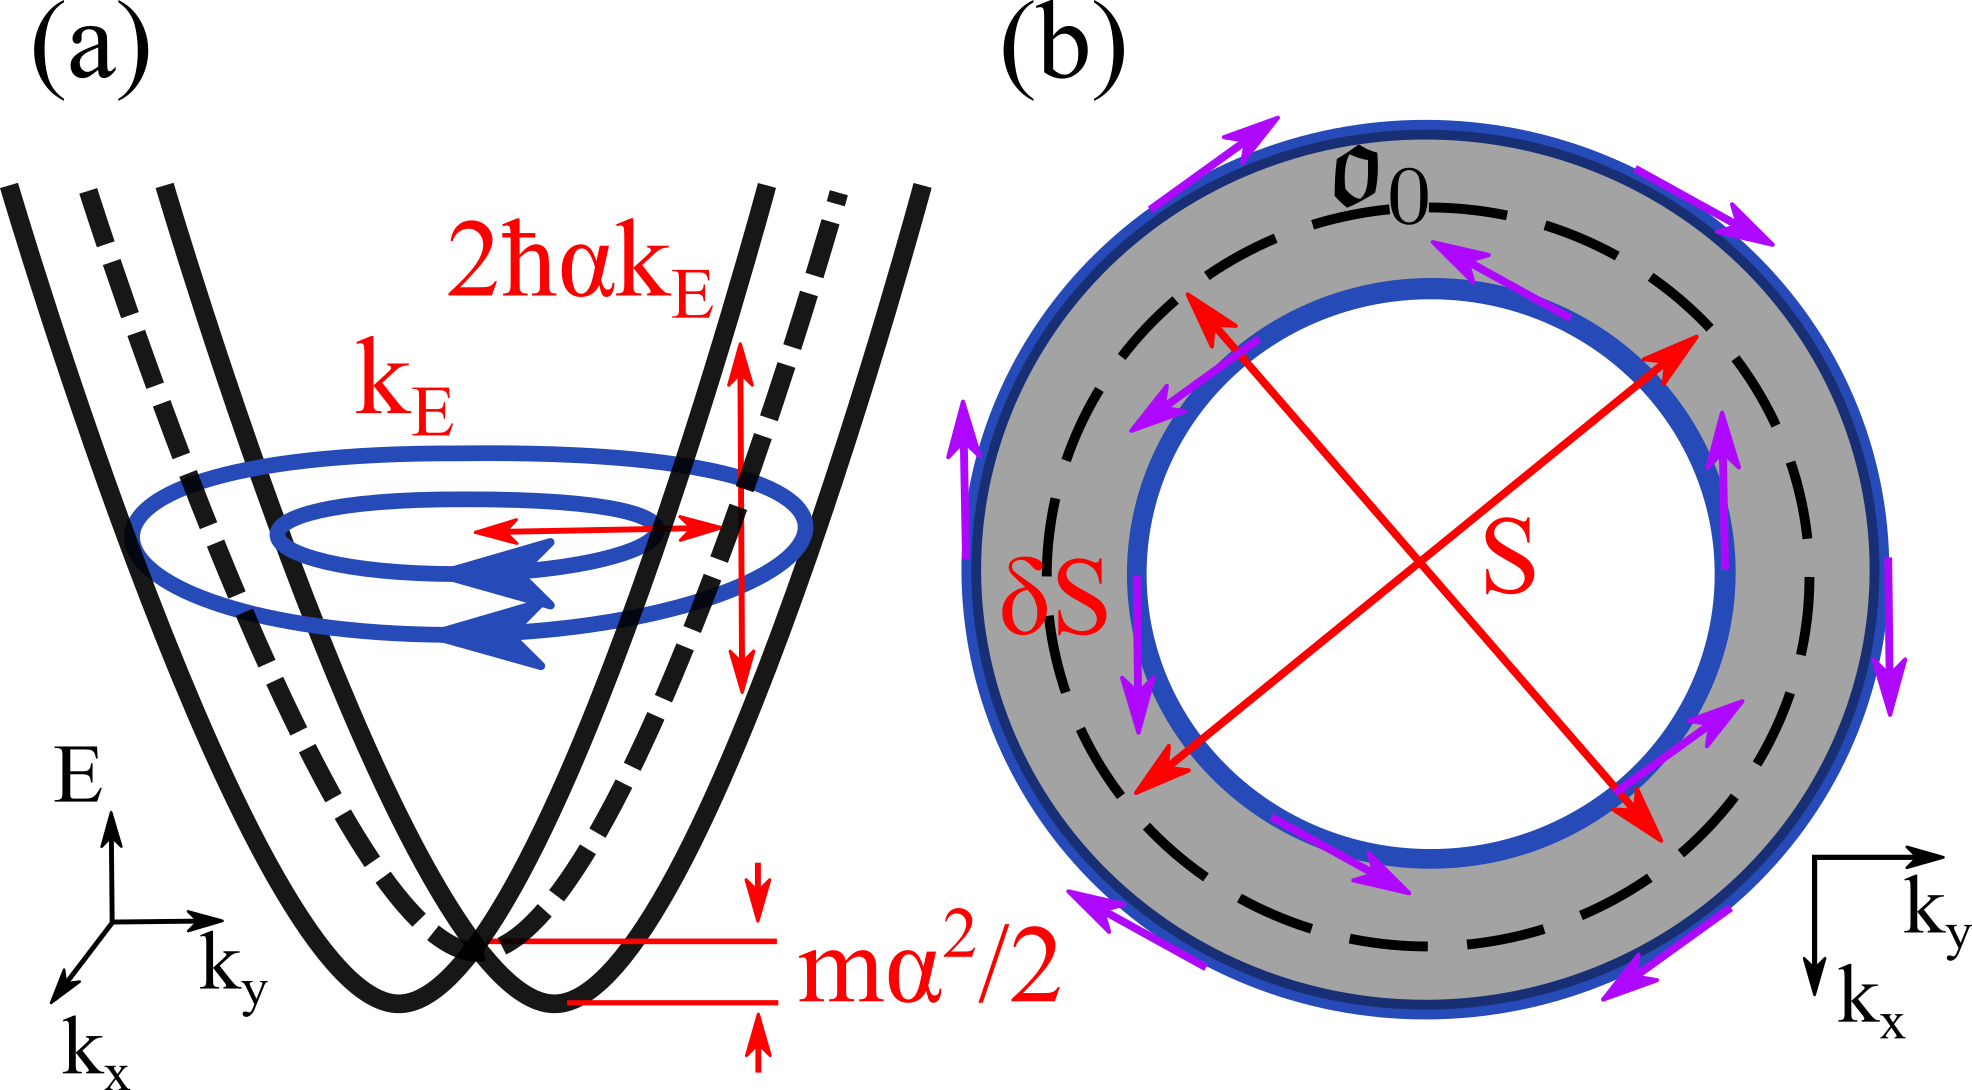
\includegraphics[width=0.8\textwidth]{../figures/orbits.png}
	\centering
	\caption{(a) 实线(虚线)阐释了具有(没有)Rashba自旋轨道耦合的二位电子气的能带色散。图中具有方向的圆代表了磁振子轨道,其中磁场方向为$-z$方向。 (b) 虚的圈$S$标注出了零阶轨道$\frako_0$;$\delta S$是自旋轨道耦合劈裂的轨道的面积之差;紫色的箭头标出了自旋结构。\label{fig:orbits}}
\end{figure}

我们的工作给出了一个适用于近简并能带的推广的量子化条件,这个量子化条件的适用范围包括具有自旋轨道劈裂的能带。我们定义近简并为磁振子面积的差远小于磁振子面积的平均值$|\delta S/S|{\ll}1$。我们提出的量子化条件还依赖于另一个条件:$S$远大于$1/l^2$,这里的$l$事磁长度$l{=}\sqrt{\hbar/eB}$;这个条件也是标准的准经典Onsager-Lifshitz-Roth理论假设。通过引入两个小量$|\delta S/S|$和$1/l^2|S|$,我们的研究推广深化了前人仅仅基于一个小量的准经典理论\cite{kohn_effham,blount_effham,rotheffham,wannier_fredkin,fischbeck_review,Mikitik_quantizationrule,topoferm,100p,gao_zero-field_2017}。

$1/l^2|\delta S|$量化了由塞曼能导致的近简并的轨道的耦合。在$l^2|\delta S|{\gg}1$的情况下,Onsager-Lifshitz{-Roth}量子化条件可以分别作用在两个共心但是不耦合的磁振子轨道。在另外一个极限$l^2|\delta S|{\ll}1$,自旋轨道耦合导致的劈裂可以忽略,我们可以采用已有的严格简并能带的量子化条件\cite{rotheffham,rothmag,topoferm,100p,Mikitik_quantizationrule}。我们的统一的量子化条件给出了介于前述的两个极限情况下的朗道能级的解($l^2|\delta S|{\sim}1$),这种情况下,塞曼能和自旋轨道耦合的能量基本相同;而前人的工作仅仅展示了这两个能量一个远大于另一个的情况下的量子化条件。我们工作给出了在任意对称群的具有自旋轨道耦合的晶体的量子化条件。章节\ref{sec:qtznrules}描述了这个近简并能带的量子化条件,其中哦我们假设了一个自旋二分之一(或者赝自旋二分之一)的自由度。正如章节\ref{sec:discussion}所述,我们的量子化条件能够涵盖任意带数的近简并能带的朗道量子化。


在章节\ref{sec:Rashba}中,我们利用具有Rashba和Dresselhaus自旋轨道耦合的二维电子气,证明了我们的量子化能级的有效性。如果给具有Rashba自旋轨道耦合的二维电子气加上足够强的面内磁场,能带中的Dirac点不仅仅会移动,而且会倾斜,成为一个第二类的狄拉克点\cite{soluyanov_type-ii_2015, muechler_tilted_2016, bergholtz_topology_2015}。在章节\ref{sec:inplanezeeman}中,我们研究了第二类狄拉克点附近的Landau-Zener隧穿现象。特别的,我们将要证明我们的量子化条件囊括了近简并能带之间的量子隧穿,这个现象被称为带间的磁隧穿\cite{kaganov_coherent_1983,slutskin_dynamics_1968,AALG,100p}。我们将要认真研究一个最近提出的二类狄拉克点附近的完美Klein隧穿的现象\cite{obrien_magnetic_2016},我们发现如果考虑了塞曼效应的话,这个完美隧穿永远不会发生。


\section{量子化条件\label{sec:qtznrules}}

首先让我们大致解释一下这个量子化条件是怎么出现的;我们将这个量子化条件的分步的严格的证明留到附录\ref{app:quantizationruleproof}中。我们要考虑的是一个没有加磁场的时候有着离散平移不变性的哈密顿量: $\hat{H}_0{+}\delta \hat{H}$。前面的这个分解要求$\hat{H}_0$的能带在每一个波矢$\bk$处是$D$重简并的,而$\delta \hat{H}$则作为微扰破除这个$D$重简并。简单起见,我们假设$D{=}2$的自旋简并,$D>2$的情形则留在附录\ref{app:quantizationruleproof}中讨论。一个简单的例子是$\hat{H}_0$是薛定谔哈密顿量,而$\delta \hat{H}$是自旋轨道耦合的哈密顿量;另一个例子是$\hat{H}_0$是具有空间反演的包含自旋轨道耦合的泡利哈密顿量,而$\delta \hat{H}$是一个晶格畸变,轻微破坏了空间反演对称性。

现在让我们加上一个磁场,我们首先考虑忽略$\delta \hat{H}$和塞曼效应的自旋简并的朗道能级。在准经典的描述下,我们对$\hat{H}_0$的低能简并的能带的磁场动力学性质进行考察,这条能带的色散记为$\var(\bk)$。比如说,对于Rashba模型,$\var(\bk){=}\hbar^2 k^2/2m{+}\order(k^4)$。众所周知,朗道量子化是由Peierls修正得到的$\var(\bk){\rightarrow}\var(\bK)$\cite{peierls_substitution},这里的$\boldsymbol{K}{:}{=}\boldsymbol{k}{+}(e/\hbar) \boldsymbol{A}(i\nabla_{\boldsymbol{k}})$,并且$\boldsymbol{A}(\br)$是矢势。我们假设磁场沿着$-z$方向,$[K_x,K_y]{=}i\lmt$。准经典的波函数的解对应着电子在$\var(\bk)$的等能面作回旋运动【见图\ref{fig:orbits}(b)】,这个蕴含着电子运动方向(运动方程为$ \hbar dk_{\alpha}/dt {=} \lmt \epsilon_{\ab}\partial \var/\partial k_{\beta} $,其中 $\epsilon_{xy}{=}{-}\epsilon_{yx}{=}1$)的轨道被称为零阶轨道$\frako_0$。在这个工作中,我们仅仅关注闭合的轨道,闭合的意思指的是轨道不会横穿布里渊区。

朗道能级的量子化条件反映了WKB准经典波函数在轨道$\frako_0$上的单值性\cite{berry_mount_review},换句话说,电子在一个磁振子周期$T_c$中获得的相位是$2\pi$的整数倍:$(l^2S(E){+}\gamma)/2\pi{\in}\Z$。最高阶的相位是是$l^2S{:}{=}{-}l^2\int_{0}^{T_c} k_x \dot{k}_y dt$;$S$同时也可以阐释为具有正负号(对于电子型的轨道是正的)的$\bk$空间$\frako_0$的面积,见图\ref{fig:orbits}(b)。$\gamma$是第二阶的Maslov相位修正\cite{keller1958},这个修正等于$\frako_0$绕的圈数$r$乘以$\pi$,也就是切向量的绕圈数)\cite{100p};对于一个能够连续变化为圆的轨道,$r{=}{\pm} 1$。在零阶近似下,所有的朗道能级是自旋简并的,能级间隔是
\e{ \var_c:=\f{2\pi}{l^2|\partial S/\partial E|}:=\f{\hbar^2}{ml^2}:=\f{h}{T_c}. \label{def:cyclotron}}
这里,$\var_c$和$T_c$分别是零阶轨道的磁振子能量和周期,$m$是有效质量。下面开始,朗道能级的简并指的就是自旋简并。



当我们考虑一阶效应的时候,$\delta \hat{H}$和塞曼效应会导致一个一阶的相位修正($\lambda_a$),这个相位修正一般而言对两个不同的自旋态是不同的(我们用$a{=}1,2$标记):
\begin{equation}
l^2S(E)+\lambda_a(E,B)+\gamma=2\pi n,\as  n\in \mathbb{Z},\;a=1,2. \label{eq:rule}
\end{equation}
这表示朗道能级的自旋简并被破除,朗道能级之间的间隔是$\var_c|\lambda_1{-}\lambda_2|/2\pi$。相位修正$\lambda_a$可以看成一个时间周期性的,微扰性的哈密顿量($\calh$)的Floquet准能量\cite{shirley_solution_1965},这个哈密顿量控制着自旋波函数的演化。$\lambda_a$是下面路径有序的指数积分的本征值$\{e^{i\lambda_a}\}_{a=1}^2$:
\begin{equation}
\A{:}{=}\overline{\exp}\left[-\frac{i}{\hbar}\int_0^{T_c} \calh(\bk(t)) dt\right],
\label{eq:prop}
\end{equation}
这里$\bk(t){\in}\frako_0$是一个时间周期性的函数,由运动方程决定。$\calh$是一个$2\times 2$的矩阵:
\begin{equation}
\calh=\delta \var +B\bigg(M_z -g_s\mu_{B}\f{s_z}{\hbar} + e\epsilon_{\alpha\beta}\mathfrak{X}_{\beta}v_{\alpha}\bigg):=\delta \var+B\calm,\label{eq:H1}
\end{equation}
$\delta \var$是$\delta \hat{H}$在$\hat{H}_0$的简并子空间(也就是前述的两条简并的带)中的投影。出于简单起见,我们假设$\delta \var$的迹是零;如果 $\delta\hat{H}$是一个自旋轨道耦合的哈密顿量,那么$\delta \var$的迹是零是得到保证的。更一般的情况下,我们总可以将$\delta \hat{H}$的投影的有迹的部分吸收到$\var(\bk)$的定义里去。在劈开的能带里(我们将这两个能带标记为${+}$和$-$,其中$+$是外面的轨道,$-$是里面的轨道),$\delta \var$是一个对角的矩阵,其对角元($\delta \var_+,~\delta \var_-{=}{-}\delta \var_+$)和耦合参数相关
\e{-\int_0^{T_c} (\delta \var_+{-}\delta \var_-) \frac{dt}{\hbar} \approx l^2\delta S. \label{spinsplitwkb}}

式\ref{eq:H1}中剩下的项可以看成一个广义的塞曼作用项$B\calm$,这一项正比于$B$,是Peierls-Onsager哈密顿量$\var(\bK)$的一阶修正\cite{rotheffham,blount_effham,kohn_effham}。这个广义的塞曼作用项包括近简并能带的自旋的塞曼作用能($g_s\mu_Bs_z/\hbar$)和轨道磁矩($M_z$)的塞曼作用能\cite{thonhauser_orbital_2005};轨道磁矩可以用布洛赫波$\psi_{n\bk}$之间的速度矩阵元表示出来$\boldsymbol{\Pi}_{mn}=i\langle\psi_m|[\hat{H}_0, \hat{\boldsymbol{r}}]|\psi_n\rangle/\hbar$:

\e{
	[M_z]_{mn}=\f{ie\hbar}{2}\sum_l'\f{\Pi_{x,ml}\Pi_{y,ln}-\Pi_{y,ml}\Pi_{x,ln}}{\epsilon_m-\epsilon_l}. \label{eq:orbitalmoment}
}
这里,对$l$的求和不包括这两条近简并的能带。最后,广义的塞曼作用项还包括一个几何相位的贡献,这一个贡献可以用$2\times 2$的非阿贝尔的贝里联络\cite{berry_quantal_1984,wilczek_appearance_1984}和零阶的能带速度表达出来
\e{\mathfrak{X}_{\beta,mn}{=}i\braket{u_m}{\partial u_n/\partial k_{\beta}},  \;\;\;v_{\alpha}:= \f{1}{\hbar}\p{\var}{k_{\alpha}},\label{berryconn}}
这里$\{u_n\}_{n=1}^2$是布洛赫波的周期性部分。

式\ref{eq:rule}至\ref{berryconn}能够让我们将$\lambda_{1,2}$计算到$1/l^2|S|$和$|\delta S/S|$的最低阶,这些式子对任意有限的$l^2|\delta S|$和$|B\calm|/\delta \var_{\pm}$都是有效的。值得指出的式,我们提出的量子化条件相对于近简并能带构成的子空间内的幺正变换是不变的(见附录\ref{app:quantizationruleproof})。在下面的讨论中,如果可能的话,有的时候采用一个和$\bk$无关的基来表达$\calh$更加方便,这种情况下,非阿贝尔的贝里联络这组基下面为零。

\subsection{在两种极限情况下恢复到Onsager-Lifshitz量子化条件}\label{sec:recoveronsager}

现在,我们用近简并的能带(用$\pm$标志)作基,讨论一下$\delta \var$和$B\calm$相互之间的大小关系。我们将要证明,在其中一个远大于另外一个的情况下,我们提出的量子化条件会恢复到已有的针对独立轨道或者简并轨道的Onsager-Lifshitz-Roth量子化条件。

\noi{i} 如果$|\var_+{-}\var_-|$在$\frako_0$的每一个点都远大于$B|\calm_{+-}|$。在这样的情况下,电子在磁场下将会进行绝热(也就是维持在同一个能带的)运动\cite{nenciu_review},此时两个轨道可以看成非简并并且独立的。在$B{\rightarrow} 0$的情况下,如果两条近简并的能带没有交上的话,电子的运动始终会退化为绝热运动。(有的时候近简并的能带会交上,一个例子就是二类狄拉克点,这个例子将在小节\ref{sec:inplanezeeman}和小节\ref{sec:rotsymmbreakdown})在这样的情况下,我们可以忽略带间跃迁的矩阵元$B\calm_{+-}$,此时$\cala$成为一个对角的矩阵,对角元$e^{i\lambda_{\pm}}$为
\e{\lambda_{\sma{\pm}} = -\int_0^{T_c}\calh_{\sma{\pm\pm}}\f{dt}{\hbar}=\pm \f{1}{2}l^2\delta S - B\int_0^{T_c}\calm_{\sma{\pm\pm}}\f{dt}{\hbar}.  \label{phaseindependentorbit}}
式\ref{eq:rule},以及式\ref{phaseindependentorbit},和前人的针对独立,非简并的面积为$S{\pm}\delta S$的两个轨道的Onsager-Lifshitz量子化条件是一致的\cite{Onsager,lifshitz_kosevich,lifshitz_kosevich_jetp}。这个独立轨道的量子化条件包含了首先由Roth\cite{rothmag}提出的相位修正。如果我们微扰地加进$B\calm_{\sma{+-}}$,$\lambda_{\pm}$ (参见 式\ref{phaseindependentorbit})可以表达为$B$地洛朗级数,并且最低阶项时$1/B$;这一点将会在下面地样例讨论(参见式 \ref{lambdasmallB})中设计,并且会被用来解释量子振荡的多种现象(参见节\ref{sec:qo})。


\noi{ii} 让我们现在讨论广义的塞曼能$B\calm$远大于$(\delta \var_+{-}\delta\var_-)$的情况。式\ref{eq:rule}至\ref{berryconn}以及$\calh{\approx}B\calm$,和我们之前的工作中\cite{topoferm,100p}得到的任意对称性的简并轨道的量子化条件是一致的。


由式\ref{eq:rule}至\ref{berryconn}总结出来的量子化条件,是本章的理论性的进展,本章下面的内容主要关注这个量子化条件会带来什么样的物理现象。我们首先要在绝热近似失效的时候(也就是$\delta \epsilon$和$B\calm$的大小相互竞争的时候)证明我们的量子化条件的有效性,这包括两种情况:(i)如果自旋劈裂的轨道在连续旋转变换下不变(比如说Rashba二维电子气模型),那么绝热近似在整个轨道都会失效(参见节\ref{sec:Rashba})。(ii)如果自旋劈裂的轨道是不对称的,绝热近似有可能在某一个孤立的点失效,一个简单的例子就是能带在第二类狄拉克点处相交(参见节\ref{sec:inplanezeeman})。在节\ref{sec:llquasideg}中,我们将要讨论多少个实的参数才能够调节得到$\lambda_1{=}\lambda_2$(mod $2\pi$),这个式子等价于朗道能级的近简并。


\section{案例研究:任意方向磁场中的Rashba二维电子气}

\subsection{面外磁场中的Rashba二维电子气}\label{sec:Rashba}

在这一节里,我们将要将我们的量子化条件应用于Rashba模型(参见式\ref{eq:Rashba-Hamiltonian}),这种情况下,简单的解析的朗道能级的解式存在的,可以和我们的量子化条件做对比\cite{bychkov_oscillatory_1984}。

出于简单起见,我们认为式\ref{eq:Rashba-Hamiltonian}中的泡利矩阵对应的就是自旋:$s_i{=}\hbar \sigma_i/2$。我们来计算半径为$k$的磁振子轨道$\frako_0$上的有效哈密顿量$\calh(\bk)$。用Rashba哈密顿量$H_R$(参见式\ref{eq:Rashba-Hamiltonian})的能带作基
\e{\calh(\bk)=-\hbar\alpha k\tau_z{+}\f{g_{s\perp}}{2}\mu_{\sma{B}}B\tau_x {-} \f{eB\hbar}{2m} (\tau_x-I) \epsilon_{\alpha\beta} k_{\alpha}\nabla_{\beta}\theta,\label{rashbaeffham}}
这里$\tau_i$是一套新的泡利矩阵,$\tau_z{=}{+} 1$ 和 ${-}1$ 分别对应的是外轨道和内轨道。 $e^{i\theta_{\bk}}{=}(ik_x{-}k_y)/k$是面内的$H_R$的自旋劈裂场$(-\hbar\alpha k_y,\hbar\alpha k_x,0)$的角度(参见式 \ref{eq:Rashba-Hamiltonian}),这个自旋劈裂场在$\frako_0$上转了一圈;由于我们基的自旋平行(或者反平行)于自旋劈裂场,因此也转了一圈【参见图\ref{fig:orbits}(b)】。上式中正比如自旋旋转速度($\nabk \theta$)的项来自于非阿贝尔的贝里联络。$\calh$的第一项对应于自旋轨道耦合引起的劈裂;其余项可以认为是磁场导致的能带变形。轨道磁矩$B M_z$一般而言会混合近简并的两个带和其余的所有能带,在这里这个效应被吸收在有效的$g$因子中$g_{s\perp}$。众所周知,塞曼效应一般会让自旋朝向磁场$\bB$的方向;令人惊异的是,非阿贝尔的贝里相位在这里也有一个自旋极化的效应,但是和塞曼效应方向相反。这两个效应在自由电子的时候完全抵消($g_{s\perp}=2$以及 $m$等于自由电子质量$m_0$),这个抵消一般不发生在能带电子上。

由于$H_R$的连续旋转对称性的存在,$\nabk \theta$的大小是$1/k$,并且和$\frako_0$相切;因此,$\calh$在$\frako_0$上是一个常数,而传播子则化简为不需要路径有序的$\cala{=}e^{{-}i\calh T_c/\hbar}$,因此量子化条件的相位修正仅仅是$\calh$的本征值乘以$T_c$:
\begin{equation}
\lambda_{\pm}=\pm\f1{2}\sqrt{({l^2\delta S})^2+\pi^2(g_{s\perp}m/m_0-2)^2}+\pi. \label{eq:Rashba-lambda}
\end{equation}
这是一个面积差$\delta S$(参见式\ref{deltaSvsS})和有效质量$m$的函数。多出来的$\pi$来自于单带的贝里相位,体现在$\theta_{\bk}$绕了${\pm}2\pi$。两个在根号下面的量来自于自旋轨道耦合导致的轨道劈裂$\delta \var$以及(在零场的能带基下的)$B\calm$的带间矩阵元。

在弱耦合极限下,$l^2\delta S \gg \pi|g_{s\perp} m/m_0{-}2|$,我们可以将式\ref{eq:Rashba-lambda}展开为$B$的洛朗级数:
\e{\lambda_{\pm}= \pm \f{l^2\delta S}{2} +\pi \pm \f{\pi^2}{4}\f{(g_{s\perp}m/m_0-2)^2}{l^2\delta S} + O(B^2). \label{lambdasmallB}}
式\ref{eq:rule}以及式\ref{lambdasmallB}的右手边前两项,也可以从标准的针对独立轨道的Onsager-Lifshitz量子化条件导出,其中$\pi$来自于贝里相位的修正:$l^2(S{\pm}\delta S)/2\pi {\in}\Z$。更高阶的项则来自于磁场导致的能带之间的混合。Mineev在Rashba模型下得到了式\ref{lambdasmallB}中的一部分\cite{mineev_haas--van_2005};由于没有考虑带间的贝里联络,他漏掉了$(g_{s\perp}m/m_0-2)$中的第二项(参见式\ref{lambdasmallB})。

在强耦合极限,也就是$l^2\delta S {\ll}\pi(g_{s\perp}m/m_0{-}2)$的情况下,$\lambda_{\pm}{\approx}{\pm}\pi g_{s\perp}m/2m_0$ mod $2\pi$,这对应着没有自旋轨道耦合的情况下,朗道能级劈裂了$g_{s}\mu_BB$。

我们的量子化条件【式\ref{eq:rule}和\ref{eq:Rashba-lambda}】可以和已知的Peierls替换过的哈密顿量(加上自旋塞曼效应)的精确解进行比对。精确解\cite{bychkov_oscillatory_1984}可以通过下式得出:
\e{
	&n_{\pm}=\frac{l^2S}{2\pi}+\frac{l^2\delta S}{16\pi}\f{\delta S}{S}\lin 
	&\pm\f1{2}\sqrt{\bigg(\frac{l^2\delta S}{8\pi}\f{\delta S}{S}\bigg)^2+(l^2\delta S)^2+\pi^2\bigg(\f{g_{s\perp}m}{m_0}-2\bigg)^2},\label{eq:Rashba-exact}}
这里的$\delta S(E)$和$S(E)$的形式参见式\ref{deltaSvsS};$n_{+}{\ge} 1$和$n_-{\ge} 0$是整数的朗道能级的标号,$\pm$代表两套朗道能级。在近简并的($\delta S/S\ll 1$)准经典的($1/l^2S \ll 1$)情况下,在$l^2\delta S$是有限的时候,式\ref{eq:Rashba-exact}里面的$\delta S/S$项可以忽略,于是式\ref{eq:Rashba-exact}就退化为我们的量子化条件,其中$\lambda_{\pm}$由是\ref{eq:Rashba-lambda}给出。


我们进一步给$H_R$加上Dresselhaus自旋轨道耦合,在这样的情况下,据我们所知,朗道能级的严格解析解是不存在的。这种情况下,我们可以通过数值对角化来验证我们的量子化条件的可靠性,这一部分内容在附录\ref{app:approximatevsexact}中。

\subsection{磁隧穿的案例研究:倾斜磁场中的Rashba二维电子气}\label{sec:inplanezeeman}

我们的下一个案例研究是一个(接近)相交的二类狄拉克点\cite{soluyanov_type-ii_2015,muechler_tilted_2016}。二类狄拉克点是传统狄拉克点的一个变种,其区别在于二类狄拉克点的能带色散不是对称的。在二类狄拉克点附近的量子隧穿数学上和Landau-Zener隧穿是一致的,仅仅是电场力变成了洛伦兹力\cite{AALG,obrien_magnetic_2016,kane_blount}。这里,我们将要证明Landau-Zener动力学很自然的可以从我们的量子化条件得出(式\ref{eq:rule}到式\ref{eq:H1})我们将要研究电子的运动会怎么受到塞曼效应的影响。特别地,我们将会展示O'Brien等人预言的\cite{obrien_magnetic_2016}完美的Klein透射在考虑进塞曼效应之后,并不是真正地完美。

我们再次从Rashba模型出发(参见式\ref{eq:Rashba-Hamiltonian}),它有一个旋转对称的狄拉克点。要将这个狄拉克点变成二类的,我们引入一个面内的磁场$B_\parallel$(平行于$y$方向)导致的塞曼项:
\e{ 
	H_{RZ}=\f{{\hbar^2}k^{2}}{2m}+\delta \var; \;\;\;\delta \var=d_x\sigma_x+d_y\sigma_y,\lin
	(d_x,d_y):=(-\hbar\alpha k_y,\hbar\alpha k_x+\zpar),\;\;\;\zpar:= g_{s\parallel} \mu_B B_{\parallel}/2.
	\label{eq:RZ-Hamiltonian}}
尽管这一项同时破坏了时间反演($T$)和二重旋转($\rot_2$),他们的乘积($\rot_2 T$)还是哈密顿量的对称性,这一点体现在 $\sigma_x H^*_{RZ}(\bk)\sigma_x{=}H_{RZ}(\bk)$, 并且让每个$\bk$的自旋严格躺在面内。二维情况下,在这个对称群中,狄拉克点可以移动,但是不能够打开能隙。面内的塞曼场不仅挪动了狄拉克点的位置到
\begin{eqnarray}
\bar{k}_x & = & -\frac{\zpar}{\hbar\alpha},\;\bar{k}_y=0,\;\epsilon_{0}=\frac{\zpar^{2}}{2m\alpha^2},\label{whereisdiracpoint}
\end{eqnarray}
而且将狄拉克点的能带倾斜了过来。如果我们在狄拉克点附近线性化这个哈密顿量,我们就可以看到这个倾斜
\e{
	H & =\hbar\alpha\left[\left(\sigma_y-\frac{\zpar}{m\alpha^2}\right)\delta k_{x}-\sigma_{x}\delta k_{y}\right]+\epsilon_{0}.}
当$|\zpar|>|m\alpha^2|$的时候,狄拉克锥在$x$方向倾斜角度超过了90度,进而导致等能线的Lifshitz相变。在线性近似下,等能线从圆形变成了双曲线,这一点体现在图\ref{fig:RZ}(a)中。一个倾斜超过九十度的狄拉克锥就是第二类的狄拉克锥。我们的案例研究就是要研究两个电子口袋连接在一起的第二类狄拉克点(参见图\ref{fig:RZ}(a,b)),这个案例研究和前人的不同\cite{obrien_magnetic_2016,AALG},前人研究的第二类狄拉克点是电子和空穴口袋之间相交得到的。

\begin{figure}
	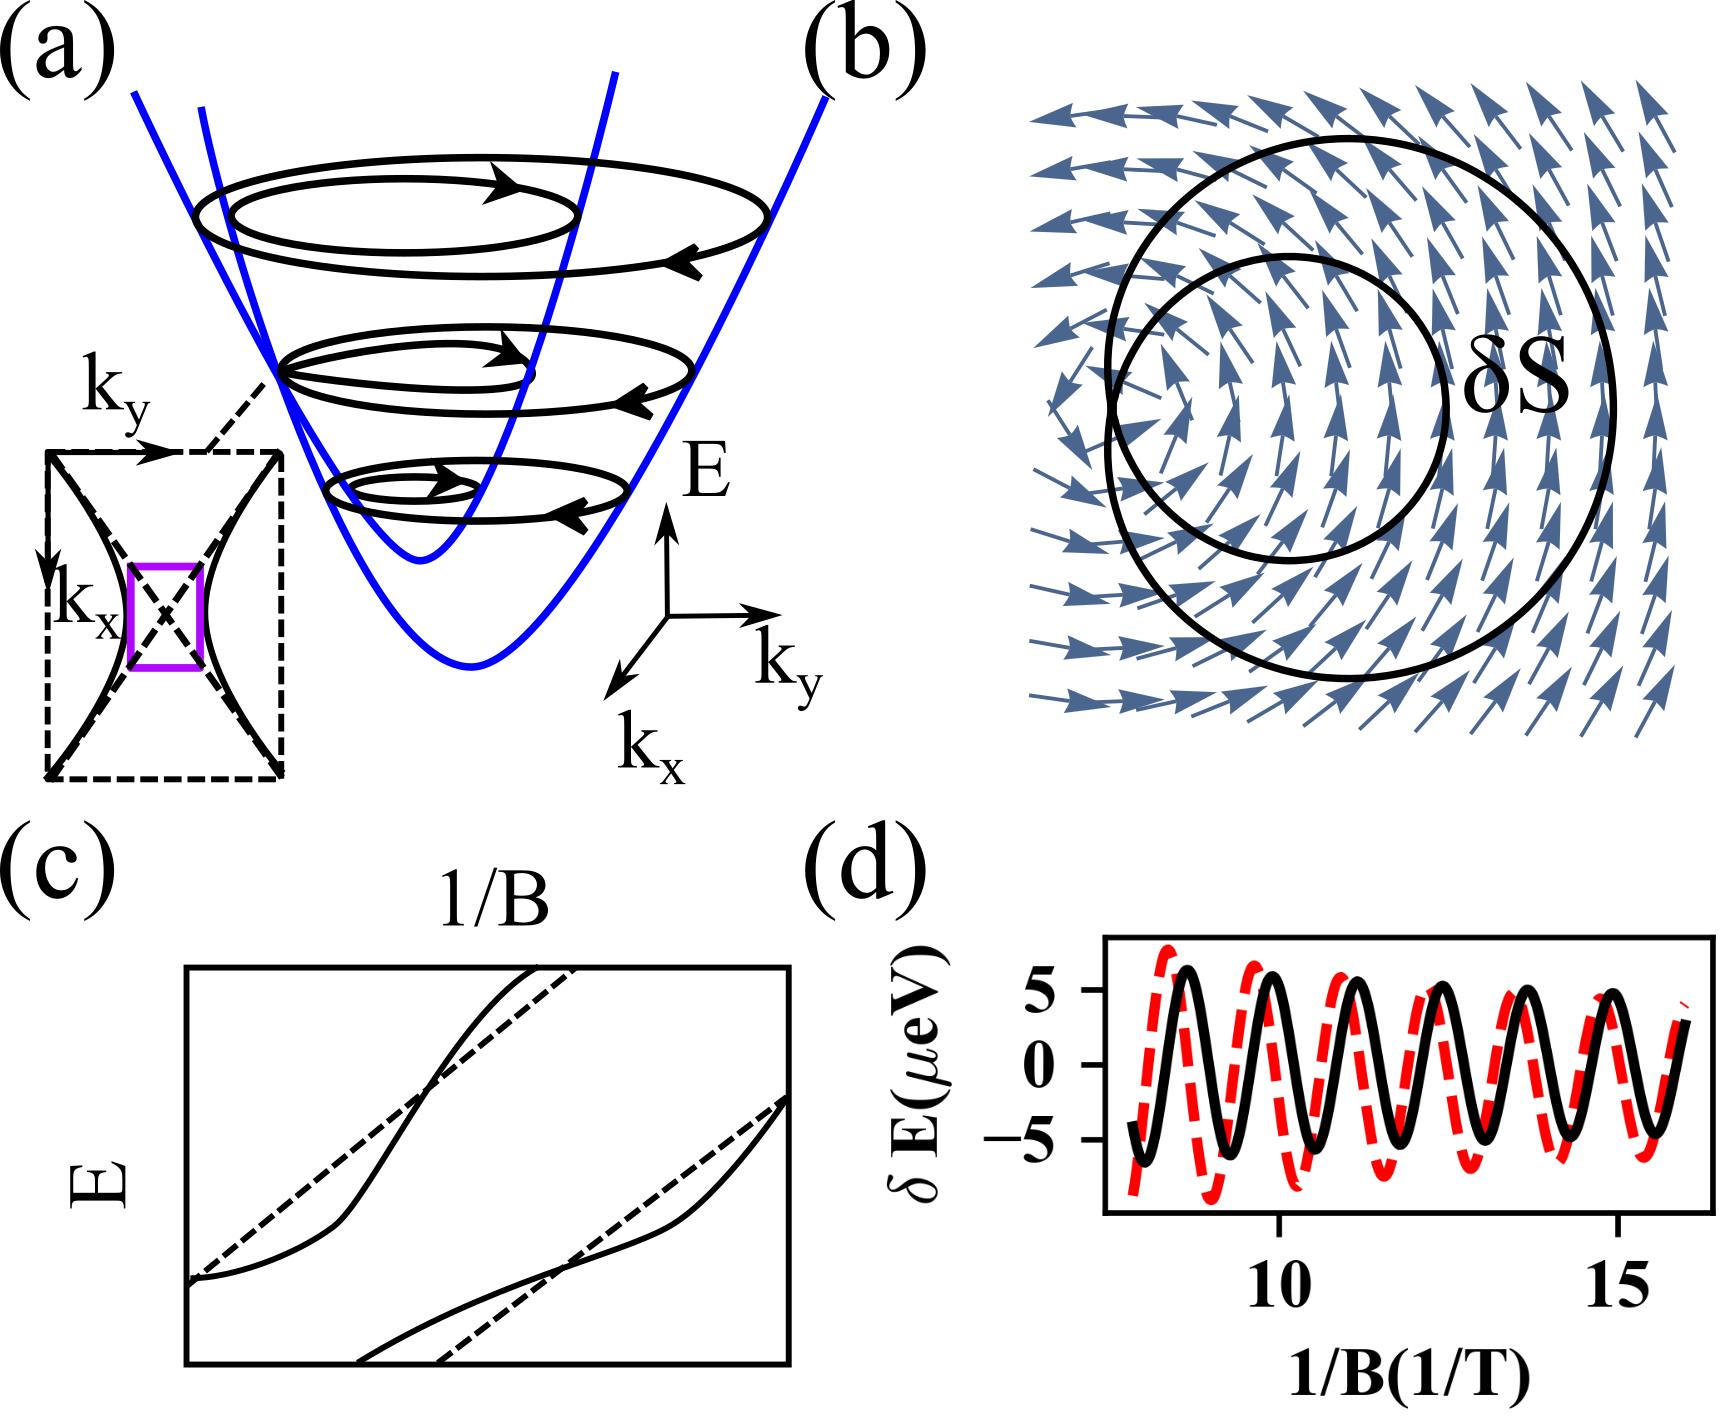
\includegraphics[width=0.8\columnwidth]{../figures/RZ.png}
	\centering
	\caption{(a)展示了Rashba二维电子气在倾斜磁场中的磁振子轨道。内嵌的图展示了第二类狄拉克点的放大图。(b)展示了能量正好在第二类狄拉克点的时候的磁振子轨道。一个能够Klein透射的电子将会沿着这个莫比乌斯环形的轨道运动。这个图片的背景是自旋劈裂场的方向($d_x,d_y$),自旋劈裂场导致了原先的能带$\delta\var$的能量劈裂(参见式\ref{eq:RZ-Hamiltonian}。内(外)圈的波函数的自旋是平行于(反平行于)自选劈裂场的。(c)在弱耦合情况下,演示了在第二类狄拉克点附近的朗道能级。虚线是莫比乌斯轨道的Onsager-Lifshitz-Roth量子化能级(参见式\ref{trefoilrule}),实线则包含了隧穿导致的的一阶修正(参见式\ref{RZfirstorderE}) (d) 黑色的实线是$\delta E_n$(参见式\ref{RZfirstorderE}),也就是由于不是完美Klein透射导致的能量修正;作为对比,红色的虚线是数值严格对角化得到的相应的能量修正。这个图采用了最接近0.45eV的朗道能级,并且采用了偶数$n$;在我们采用的参数下 ($m{=}0.076m_0$, $\alpha{=} 1.5\times10^{5}$cm/s, $Z_\parallel {=}$1meV 以及 $g_{s\perp}=2$),二类狄拉克点在 0.5eV处。 
	\label{fig:RZ}}
\end{figure}

在面内的磁场以外,我们再加入一个面外的磁场$B_{\perp}$,其磁长度为$\lper{=}\sqrt{\hbar/eB_{\perp}}$,磁振子能量为$\var^{\sma{\perp}}_c{:}{=}\hbar^2/m\lper^2{:}{=}\hbar \omega_c^{\sma{\perp}}{:}{=}h/T_c^{\sma{\perp}}$,自旋塞曼效应为$\zper{:}{=}{g_{s\perp}}\mu_B B_{\perp}/2$。我们在这里假设$1/\lper^2S{\ll}1$,这里$S$是零阶轨道(有效质量为$m$半径为$k_E{=}\sqrt{2mE}/\hbar$)。对于远高于$m\alpha^2$和 $\zpar$的能量,近简并条件($\delta S/S{\ll}1$)是满足的,这里$\delta S$是自旋轨道和耦合和面内的塞曼场导致的磁振子轨道的面积差(参见图\ref{fig:RZ}(b))。由于$1/\lper^2S$和$\delta S/S$很小($\lper^2\delta S$是有限的),我们的量子化条件(参见式\ref{eq:rule}至式\ref{eq:H1})可以应用于这个模型,其有效哈密顿量为
\begin{equation}
\calh(t)=\hbar\alpha(k_{x}\sigma_{y}-k_{y}\sigma_{x})+Z_\parallel\sigma_{y}-Z_\perp\sigma_{z}.\label{calHRZ}
\end{equation}
这里,$t$是一个参数化零阶轨道的参数$\bk(t){=}({-}k_E \cos \omega_c^{\sma{\perp}} t, k_E \sin \omega_c^{\sma{\perp}} t)$,在和是\ref{calHRZ}动量无关的自旋基矢下,式\ref{eq:H1}中的非阿贝尔的贝里联络$\mathfrak{X}$为零,因此广义的塞曼作用$B_{\sma{\perp}}\calm$退化为对自旋的塞曼作用$Z_\perp\sigma_{z}$。

As alluded to in \s{sec:qtznrules}, the adiabatic limit of two independent orbits does not exist if the two spin-orbit-split orbits exactly intersect at a II-Dirac point. To investigate this failure of adiabaticity, let us study the Landau levels at energies close to the II-Dirac point ($\epsilon_0$). We focus first on the regime where, on average (over $\frako_0$), the energy splitting $|\delta \var_+{-}\delta \var_-|$ [cf.\ \q{eq:RZ-Hamiltonian}] is much greater than $B_\perp|\calm_{\sma{+-}}|$. Equivalently, we are in the regime where $\hbar\alpha k_{\sma{E}}{\gg}\var_c^\perp$.\footnote{The orbit-averaged energy splitting is of order $\alpha k_{\sma{E}}$ for energies near the Dirac point. $B_\perp|\calm_{\sma{+-}}|$ is simply the Berry contribution to the Zeeman interaction, and has the form of the right-most term in \q{rashbaeffham}; this term is of order $\var_c$.} This implies that the split orbits do not appreciably hybridize -- except in the vicinity of the II-Dirac point where orbits (nearly) touch.  Near this touching point (where $t{=}0$), the dynamics of a spinor electron is described by linearizing $\H$ [cf.\ \q{calHRZ}] with respect to $t$:
\e{
	\calh = -\hbar\alpha k_{E}\omega^{\sma{\perp}}_c t\,\sigma_x+(Z_\parallel-\alpha k_{E})\sigma_y-Z_\perp\sigma_z,\label{effhamIIDirac}
}
The eigenbasis of $\sigma_x$ corresponds to two diabatic levels with characteristic slope $v_d{:}{=}\hbar\alpha k_E\omega^{\sma{\perp}}_c$; near $t{=}0$, the diabatic levels anticross  due to the hybridization terms proportional to $\sigma_{y,z}$. Generally, the probability of tunneling across the hybridization-induced barrier is  $\rho^2{=}\exp(-2\pi\barmu)$, with $\barmu{=}{E_g}^2/{2v_d \hbar}$ and $E_g$ the energy gap at the center of the anticrossing\cite{wittig_landauzener_2005,lifshitz_e.m._quantum_1991}; in this context,
\e{\barmu=\frac{Z_\perp^2+(Z_\parallel-\alpha k_{E})^2}{2\hbar\alpha k_{E}\var^{\sma{\perp}}_c}, \label{mu1}}
with $2\hbar\alpha k_E$ the spin-orbit splitting at energy $E$ [cf.\ \fig{fig:orbits}(a)]. In the absence of the out-of-plane Zeeman coupling ($Z_\perp{=}0$), $\bar{\mu}$ would vanish at the energy of the II-Dirac point -- leading to unit-probability Klein tunneling, as was first proposed by Ref. \onlinecite{obrien_magnetic_2016} in a different model of the II-Dirac point. However, with a proper account of $Z_\perp$, we find instead that $\bar{\mu}$ has a nonvanishing minimum: $\bar{\mu}_{\sma{\text{min}}}{:}{=} (g_{s\perp} m/m_0)(Z_\perp/4\hbar\alpha k_{E})$, which is a product of the dimensionless effective mass and the ratio of the out-of-plane Zeeman splitting over the spin-orbit splitting. This minimum may be significant for semiconductor heterostructures (e.g.,  $g_{s\perp}m/m_0{\sim} 1$ in InAs heterostructures\cite{pakmehr_g-factor_2015}) and  for heavy-fermion systems.